% This is samplepaper.tex, a sample chapter demonstrating the
% LLNCS macro package for Springer Computer Science proceedings;
% Version 2.21 of 2022/01/12
%
\documentclass[runningheads]{llncs}
%
\usepackage[T1]{fontenc}
% T1 fonts will be used to generate the final print and online PDFs,
% so please use T1 fonts in your manuscript whenever possible.
% Other font encondings may result in incorrect characters.
%
\usepackage{listings}
\lstset{breaklines=true}
\usepackage{algorithmic}
\usepackage{amsmath,amssymb,amsfonts}
\usepackage{algorithmic}
\usepackage{graphicx}
\usepackage{courier}
\lstset{
	basicstyle=\ttfamily\linespread{1.029}\selectfont,
	breaklines=true,
	keepspaces=true,
	emph={
		fmod, is, op, ops, eq, if, pr, endfm, 
		sort, sorts, subsort, subsorts, red, reduce
	},
	commentstyle=\color{gray}\itshape,
%	commentstyle=\color{green!50!black}\itshape\footnotesize,
	morecomment=[l]{\---},
	emphstyle={\textbf},
%	aboveskip=0.8em,
%	belowskip=0.8em
}
\usepackage{booktabs, makecell}
\usepackage[linesnumbered,ruled,vlined,noend]{algorithm2e}
\DontPrintSemicolon
\usepackage{soul}
\usepackage{color}
\usepackage{multirow}
\usepackage{float}
\usepackage{subcaption}
\usepackage{physics}
\usepackage{tikz}
\usetikzlibrary{quantikz}
\usepackage{bm}
\usepackage[
	colorlinks=true,
	linkcolor=blue,
	citecolor=blue,
	urlcolor=blue
]{hyperref}
\renewcommand{\arraystretch}{1.2}
\newcommand{\comp}{\mathrel{;}}

\newtheorem{defi}{Definition}
\newtheorem{thm}{Theorem}
\newtheorem{lem}{Lemma}
\newtheorem{cor}{Corollary}
\newtheorem{exa}{Example}
\newtheorem{rem}{Remark}
\newtheorem{conv}{Convention}[section]
\renewcommand{\theconv}{\arabic{section}.\arabic{conv}}
\renewcommand{\thedefi}{\arabic{section}.\arabic{defi}}
%\renewcommand{\theexa}{\arabic{section}.\arabic{exa}}
% Used for displaying a sample figure. If possible, figure files should
% be included in EPS format.
%
% If you use the hyperref package, please uncomment the following two lines
% to display URLs in blue roman font according to Springer's eBook style:
%\usepackage{color}
%\renewcommand\UrlFont{\color{blue}\rmfamily}
%\urlstyle{rm}
%
\begin{document}
%
\title{An Algebraic Specification for Quantum Computation in Maude\thanks{This work was supported by JSPS KAKENHI Grant Numbers JP23K28060, JP23K19959, JP24K20757, JP24KK0185.}}
%
\titlerunning{An Algebraic Specification for Quantum Computation in Maude}
% If the paper title is too long for the running head, you can set
% an abbreviated paper title here
%
\author{Canh Minh Do \and
Kazuhiro Ogata}
%
\authorrunning{C.M. Do and K. Ogata}
% First names are abbreviated in the running head.
% If there are more than two authors, 'et al.' is used.
%
\institute{Japan Advanced Institute of Science and Technology (JAIST), Nomi, Japan\\
%Asahidai 1-1, Nomi, Ishikawa, Japan\\
\email{\{canhdo,ogata\}@jaist.ac.jp}}
%
\maketitle              % typeset the header of the contribution
%
\begin{abstract}
With the rapid advancement of quantum computing, formal verification of quantum systems has become an increasingly important research topic. At the same time, the algebraic specification community, particularly the Maude community, has started to show interest in quantum computing. However, a dedicated algebraic specification framework for quantum computation is still lacking. This paper introduces \texttt{|AS4QC>}, an algebraic specification for quantum computation in Maude, which provides a formal framework for modeling, symbolic and exact reasoning about, and verifying quantum systems. We employ the ring $\mathbb{D}[\omega]$ to exactly represent complex numbers in quantum computation without approximation, use Dirac's bra-ket notation to model quantum states and quantum operations, and leverage a set of laws from quantum mechanics and basis matrix operations expressed in Dirac notation to automate reasoning about quantum computation. As case studies, we use \texttt{|AS4QC>} to verify the correctness of several nontrivial quantum programs, demonstrating the effectiveness and practicality of our approach.

\keywords{algebraic specification \and quantum computation \and verification}
\end{abstract}
%
%
%
\section{Introduction}

Quantum computing has attracted significant attention worldwide, and with substantial investment from both governments and major companies, the development of large-scale quantum computers is increasingly seen as a matter of time and sustained effort. Quantum computing differs fundamentally from classical computing by exploiting principles of quantum mechanics, such as superposition, entanglement, and interference. These properties enable quantum algorithms, such as Shor’s algorithm for integer factorization and discrete logarithms~\cite{Shor@94}, and Grover’s algorithm for unstructured database search~\cite{Grover@96}, to achieve substantial speedups over their best-known classical counterparts.
However, due to the counterintuitive and probabilistic nature of quantum computation, the likelihood of programming errors in quantum programs is much higher than in classical ones. Moreover, traditional testing techniques are much less effective in the quantum setting because of nondeterminism and probabilistic outcomes inherent in quantum measurement. Consequently, formal verification is expected to play a crucial role in ensuring the reliability of quantum systems before they can be trusted in safety-critical and security-sensitive applications.

The algebraic specification community, particularly the Maude community, has started to show interest in quantum computing. However, a dedicated algebraic specification framework for quantum computation is still lacking, which makes the development of formal verification techniques for quantum systems in Maude challenging. In this paper, we present \texttt{|AS4QC>}, an algebraic specification for quantum computation in Maude, which provides a formal framework for modeling, symbolic and exact reasoning about, and verifying quantum systems. 
To develop \texttt{|AS4QC>}, we need to support algebraic representations of complex numbers, quantum states, and quantum operations, as well as automated reasoning about quantum computation.
Kliuchnikov et al. conjectured in~\cite{Vadym@13}, and Giles and Selinger later proved in~\cite{Giles@13}, that a unitary matrix can be exactly realized by a quantum circuit over the universal Clifford + T gate set if and only if all its matrix entries belong to the ring $\mathbb{D}[\omega]$. Therefore, it is promising to study the ring $\mathbb{D}[\omega]$ and its use for the exact algebraic representation of complex numbers arising in quantum computation. Accordingly, we employ $\mathbb{D}[\omega]$ to algebraically represent complex numbers in quantum computation without approximation. 
For the algebraic representation of quantum states and quantum operations, we adopt Dirac’s bra-ket notation~\cite{Dirac@93} instead of explicitly using complex vectors and matrices as in~\cite{QWIRE@17,QX@17,wecker2014,ProjectQ@18}. Dirac notation is widely used in quantum mechanics because of its succinctness and convenience, and it allows us to obtain compact representations that are well-suited to algebraic manipulation. For automated reasoning, we leverage a set of laws from quantum mechanics and basis matrix operations expressed in Dirac notation to perform quantum computation.

Maude~\cite{Clavel2007LNCS} is a high-level specification and programming language based on rewriting logic~\cite{Meseguer@12}, focusing on simplicity, expressiveness, and performance, and providing a wide range of formal analysis facilities. Therefore, we use it to develop the algebraic specification \texttt{|AS4QC>} for quantum computation. The algebraic specification allows us to use symbolic values for complex numbers, thereby enabling symbolic quantum computation, which is a major advantage of our approach.
As case studies, we use \texttt{|AS4QC>} to verify the correctness of several nontrivial quantum programs, including 
Entanglement,
Quantum Teleportation~\cite{be93}, 
Entanglement Swapping~\cite{zu93}, 
Quantum Secret Sharing~\cite{hi99},
Quantum Relay Scheme~\cite{Sheng@05},
Bidirectional Quantum Teleportation~\cite{Shima@14},
Quantum Network Coding~\cite{Satoh@12},
and Grover's Search~\cite{Grover@96}, to demonstrate the effectiveness and practicality of our approach. The algebraic specification \texttt{|AS4QC>} and case studies are publicly available at~\url{https://github.com/canhminhdo/as4qc}.

The rest of the paper is organized as follows.
Section~\ref{sect-prel} introduces basic notations from quantum computation.
Section~\ref{sect-as4qc} presents the algebraic specification for quantum computation.
%Section~\ref{sect-cs} describes the formal specification and verification of a case study in \texttt{|AS4QC>}.
Section~\ref{sect-cs} describes a case study in \texttt{|AS4QC>}.
Section~\ref{sect-exp} shows the experimental results for several case studies.
Section~\ref{sect-rw} mentions previous work and finally concludes the paper with some future directions.

%The rest of the paper is organized as follows.
%Section~\ref{sect-prel} introduces basic notations from quantum computation.
%Section~\ref{sect-as4qc} presents the algebraic specification of quantum computation.
%Section~\ref{sect-cs} presents the application of Quantum Teleportation.
%Section~\ref{sect-exp} shows the experimental results for several case studies.
%Section~\ref{sect-rw} mentions some previous work.
%Section~\ref{sect-cls} finally concludes the paper with some future directions.

\section{Basic Notations from Quantum Computation}
\label{sect-prel}
This section describes basic notations from quantum computation (refer to~\cite{nielsen2010} for more details) and assumes that the reader has some basic knowledge of linear algebra.

The state space of a quantum system is a Hilbert space $\mathcal{H}$, which is a complete complex vector space equipped with an inner product. A pure state of a quantum system is described by a unit vector written in Dirac's ket notation as $\ket{\psi} \in \mathcal{H}$. The conjugate transpose of $\ket{\psi}$ is a row vector written in Dirac's bra notation as $\bra{\psi} \triangleq \ket{\psi}^\dagger$. The inner product of $\ket{\psi}$ and $\ket{\phi}$ is written as $\braket{\psi}{\phi}$ and they are orthogonal if $\braket{\psi}{\phi}$ = 0. The outer product of them, denoted $\dyad{\psi}{\phi}$, is a linear operator that maps any $\ket{\psi'} \in \mathcal{H}$ to $\braket{\phi}{\psi'}\ket{\psi}$. The length of $\ket{\psi}$ is defined as $\| \ket{\psi} \| \triangleq \sqrt{\braket{\psi}}$. A set of vectors $B \triangleq \{ \ket{i} : i \in I \} \in \mathcal{H}$ is orthonormal if each $\ket{i}$ is normalized and every two vectors in the set are orthogonal. Furthermore, if they span the whole space $\mathcal{H}$; that is, any vector in $\mathcal{H}$ can be written as a linear combination of vectors in $B$, then $B$ is called an orthonormal basis of $\mathcal{H}$.

A qubit is a quantum system whose state space is the two-dimensional Hilbert space $\mathcal{H}_2 = \mathbb{C}^2$. The state of a qubit can be written as $\alpha \ket{0} + \beta \ket{1}$ with $|\alpha|^2 + |\beta|^2 = 1$, where $\alpha, \beta \in \mathbb{C}$, $\ket{0} \triangleq [1\ 0]^T$, and $\ket{1} \triangleq [0\ 1]^T$ with $^T$ denoting the transpose operator. The coefficients $\alpha$ and $\beta$ are called the amplitudes of this quantum state. The set $\{\ket{0}, \ket{1}\}$ forms an orthonormal basis of $\mathcal{H}_2$ and is called the computational basis. 
For multiple qubits, we use tensor products of Hilbert spaces. Let ${\mathcal{H}}_A$ and ${\mathcal{H}}_B$ be the Hilbert spaces of systems $A$ and $B$, respectively. 
The tensor product of $\mathcal{H}_A$ and $\mathcal{H}_B$ is the Hilbert space $\mathcal{H}_A \otimes \mathcal{H}_B$ (or $\mathcal{H}_{AB}$) of their composite system $AB$. It consists of linear combinations of product states $\ket{\psi} \otimes \ket{\phi}$ (often written $\ket{\psi \phi}$ or $\ket{\psi} \ket{\phi}$) with $\ket{\psi} \in \mathcal{H}_A$ and $\ket{\phi} \in \mathcal{H}_B$. Any state in $\mathcal{H}_{A} \otimes \mathcal{H}_{B}$ that cannot be written as a product state is called an entangled state. For example, the Bell (or EPR) state $\ket{\Phi^+} = \frac{\ket{00} + \ket{11}}{\sqrt{2}}$ is maximally entangled.

In quantum computing, we mainly perform two types of operations: unitary transformation (also known as quantum gates) and quantum measurement. A unitary transformation on a quantum system in the Hilbert space $\mathcal{H}$ is a linear operator $U : \mathcal{H} \rightarrow \mathcal{H}$ satisfying $UU^\dagger = U^{\dagger} U = I_{\mathcal{H}}$, where $U^{\dagger}$ is the conjugate transpose of $U$ and $I_{\mathcal {H}}$ is the identity operator on $\mathcal{H}$. After unitary transformation, a state $\ket{\psi}$ is changed to $U\ket{\psi}$ deterministically. We present the definition of some standard unitary transformations as follows.

\begin{center}
\begin{tabular}{ p{3.8cm}p{3.5cm}l }
${\rm X }= \begin{bmatrix} 0 & 1\\ 1 & 0 \end{bmatrix}$, &
${\rm Y} =  \begin{bmatrix} 0 & -i\\ i & 0 \end{bmatrix}$, &
${\rm Z} = \begin{bmatrix} 1 & 0\\ 0 & -1 \end{bmatrix}$, \\
${\rm H} =  \frac{1}{\sqrt{2}} \begin{bmatrix}
	1 & 1\\
	1 & -1
\end{bmatrix}$, & 
${\rm T} =  \begin{bmatrix}
	1 & 0\\
	0 & e^{i\pi/4}
\end{bmatrix}$, &
${\rm CX} = \begin{bmatrix} 1 & 0 & 0 & 0 \\ 0 & 1 & 0 & 0 \\ 0 & 0 & 0 & 1 \\ 0 & 0 & 1 & 0 \end{bmatrix}$.
\end{tabular}
\end{center}

A quantum measurement on a quantum system in the Hilbert space $\mathcal{H}$ is a collection of measurement operators $\{ M_m \}$ satisfying the completeness relation $\sum\limits_{m} M^\dagger_m M_m = I$. Measuring a state $\ket{\psi}$ yields outcome $m$ with probability $p(m) = \| M_m \ket{\psi} \|^2$, and the state is changed to $\ket{\psi_m} = \frac{M_{m}\ket{\psi}}{\sqrt{p(m)}}$. Note that $M_m \ket{\psi}$ is normalized by dividing by its norm $\sqrt{p(m)} = || M_m \ket{\psi} ||$, so that it becomes a unit vector.
As an example, we consider the measurement $\{M_0 = \ketbra{0}, M_1 = \ketbra{1}\}$ applied to the state $\ket{\psi} = \alpha \ket{0} + \beta \ket{1}$ with $| \alpha |^2 + | \beta |^2 = 1$. The probabilities of obtaining outcomes $0$ and $1$ are $| \alpha |^2$ and $| \beta |^2$, respectively and the state collapses to $\ket{0}$ or $\ket{1}$ accordingly. Consequently, quantum measurement changes a quantum system in a nondeterministic and probabilistic way.

The measurement involving multiple qubits is more complex. Let us consider a two-qubit system in a state $\ket{\psi} = \alpha \ket{00} + \beta \ket{01} + \gamma \ket{10} + \delta \ket{11}$ with $|\alpha|^2 + |\beta|^2 + |\gamma|^2 + |\delta|^2 = 1$.
We use the measurement $\{M_0 = \ketbra{0}, M_1 = \ketbra{1}\}$, but note that we do not normalize quantum states after each measurement.
When we measure the first qubit, one of the following will occur:
\begin{itemize}
\item the outcome 0 with probability of $p_0 = | \alpha |^2 + | \beta |^2$, collapsing the quantum state to $\alpha \ket{00} + \beta \ket{01}$, and
\item the outcome 1 with probability of $p_1 = | \gamma |^2 + | \delta |^2$, collapsing the quantum state to $\gamma \ket{10} + \delta \ket{11}$.
\end{itemize}
Next, we measure the second qubit. The possible outcomes are illustrated in the following diagram.
\[
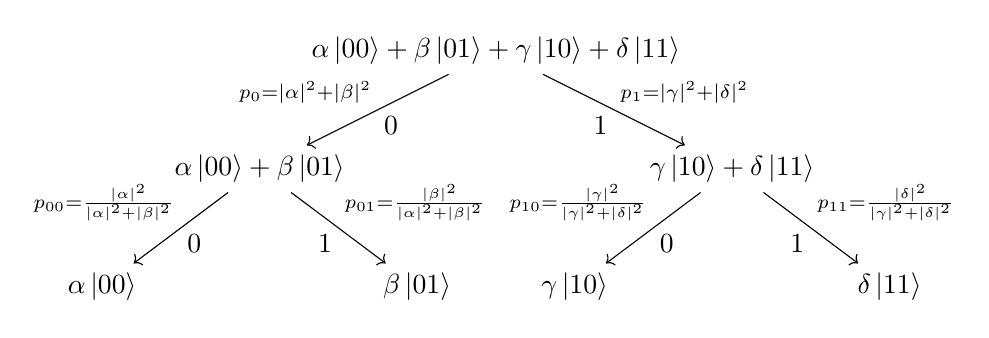
\begin{tikzpicture}[commutative diagrams/every diagram]
\node (P0) at (5,3) {$\alpha \ket{00} + \beta \ket{01} + \gamma \ket{10} + \delta \ket{11}$};
\node (P1) at (2,1.5) {$\alpha \ket{00} + \beta \ket{01}$} ;
\node (P2) at (8,1.5) {$\gamma \ket{10} + \delta \ket{11}$};
\node (P3) at (0,0) {$\alpha \ket{00}$};
\node (P4) at (4,0) {$\beta \ket{01}$};
\node (P5) at (6,0) {$\gamma \ket{10}$};
\node (P6) at (10,0) {$\delta \ket{11}$};
\path[commutative diagrams/.cd, every arrow, every label]
(P0) edge node[swap] {$p_0 = | \alpha |^2 + | \beta |^2$} node {0} (P1)
(P0) edge node[swap] {1} node {$p_1 = | \gamma |^2 + | \delta |^2$} (P2)
(P1) edge node[swap] {$p_{00} = \frac{| \alpha |^2}{| \alpha |^2 + | \beta |^2}$} node {0} (P3)
(P1) edge node[swap] {1} node {$p_{01} = \frac{| \beta |^2}{| \alpha |^2 + | \beta |^2}$} (P4)
(P2) edge node[swap] {$p_{10} = \frac{| \gamma |^2}{| \gamma |^2 + | \delta |^2}$} node {0} (P5)
(P2) edge node[swap] {1} node {$p_{11} = \frac{| \delta |^2}{| \gamma |^2 + | \delta |^2}$} (P6);
\end{tikzpicture}
\]
\noindent
In this diagram, nodes represent quantum states, and transitions are labeled with the probabilities and measurement outcomes. The total probabilities of obtaining 00, 01, 10, and 11 as the result of the two measurements are $p_0 p_{
00} = | \alpha |^2$, $p_0 p_{01} = | \beta |^2$, $p_1 p_{10} = | \gamma |^2$, and $p_1 p_{11} = | \delta |^2$. It is common to normalize quantum states to unit vectors after each measurement, ensuring that the sum of the absolute squares of the amplitudes is one. However, the diagram shows that a different normalization is more convenient. This paper adopts the normalization convention from~\cite{Selinger@04} such that each state is normalized so that the sum of the absolute squares of the amplitudes equals the total probability of reaching that state. It means that when measuring a state $\ket{\psi}$ with outcome $m$, the state changes to $\ket{\psi_m} = M_m \ket{\psi}$, which may not be a unit vector since normalization (division by its norm) is omitted. This convention significantly simplifies our representation and computation and has no effect on physical observations.
%\begin{conv}[Normalization Convention]
%\label{norm-con}
%Each state is normalized so that the sum of the absolute squares of the amplitudes equals the total probability of reaching that state.
%\end{conv}
%\noindent
%With this convention, normalizing the state after measurement is unnecessary, significantly simplifying our representation and computation. 

For each closed subspace $V$ of $\mathcal{H}$, there exists a unique projection operator $\mathcal{P}_V$. Every state $\ket{\psi} \in \mathcal{H}$ can be written as $\ket{\psi} = \ket{\psi_V} + \ket{\psi_{V^\bot}}$ with $\ket{\psi_V} \in V$ and $\ket{\psi_{V^\bot}} \in V^{\bot}$, the orthogonal complement of $V$. The projection $\mathcal{P}_V : \mathcal{H} \rightarrow V$ is defined by $\mathcal{P}_V\ket{\psi} = \ket{\psi_V}$. Since closed subspaces of $\mathcal{H}$ are in one-to-one correspondence with projection operators, we often identify $\mathcal{P}_V$ and $V$, and write $\mathcal{P}_V$ as $\mathcal{P}$ when the closed subspace $V$ is clear from context. Moreover, if a state $\ket{\psi}$ is in the closed subspace $V$ of the projection operator $\mathcal{P}_V$, then $\mathcal{P}_V\ket{\psi} = \ket{\psi}$.

\section{Algebraic Specification for Quantum Computation}
\label{sect-as4qc}

This section presents the algebraic specification \texttt{|AS4QC>} for quantum computation in Maude, including complex number representation, quantum states and quantum operations, automated reasoning about quantum computation based on a set of laws from quantum mechanics and basic matrix operations, and the usability of \texttt{|AS4QC>}. We assume that the readers are familiar with Maude.

\subsection{Complex number representation}
\label{cpx_sect}
This work focuses on symbolic and exact reasoning for quantum computation. Therefore, it is necessary to exactly represent complex numbers arising in quantum computation without approximation. Kliuchnikov et al. conjectured in~\cite{Vadym@13}, and Giles and Selinger later proved in~\cite{Giles@13}, that a unitary matrix can be exactly realized by a quantum circuit over the universal Clifford + T gate set, possibly using one additional ancilla, if and only if its matrix entries belong to the ring $\mathbb{D}[\omega]$, consisting all complex numbers of the form
$\frac{1}{{\sqrt{2}}^k}(a + b\omega + c\omega^2 + d\omega^3)$, where $k \in \mathbb{N}, a,b,c,d \in \mathbb{Z}$, and $\omega = e^{i\pi/4} = {\rm cos}(\pi/4) + i\ {\rm sin}(\pi/4) = (1 + i) / \sqrt{2}$. Using the ring $\mathbb{D}[\omega]$, a complex number is algebraically represented by a quadruple $(a, b, c, d)$ of integers and a normalization factor $k$ of a natural number. Although $\mathbb{D}[\omega]$ does not include all complex numbers, it forms a dense subset of complex numbers such that any complex number can be approximated to arbitrary precision by an element of the ring $\mathbb{D}[\omega]$~\cite{Zulehner@19}. Moreover, the subset of complex numbers is sufficient to describe various standard quantum gates. Our algebraic specification currently supports X, Y, Z, H, S, T, Rx[$\pi/2$], Ry[$\pi/2$], Rz[$\pi/2$], CX, CY, CZ, SWAP, CCX, CCY, CCZ, MCX, MCY, MCZ, MCSWAP, which already includes the universal Clifford + T gate set.
This algebraic representation of complex numbers is also sufficient to exactly represent all reachable states of OpenQASM circuits\,\footnote{OpenQASM (open quantum assembly language) is an imperative programming language for describing quantum circuits used by IBM.} when the initial state is a basis state because complex numbers in the ring $\mathbb{D}[\omega]$ are closed under addition and multiplication.

We employ the ring $\mathbb{D}[\omega]$ to algebraically represent complex numbers and also assume that all amplitudes of a quantum state share a common normalization factor $k$ as in~\cite{AutoQ@23,AutoQ@25}.  Rather than storing this factor for each amplitude, we store a single global value $k$ for the whole quantum state. The value of $k$ can be inferred from the fact that the sum of probabilities over all basis states is one. 
Moreover, the initial quantum state is usually a basis state, $k$ is initialized to zero in most cases. For each application of an H, Rx[$\pi / 2$], Ry[$\pi / 2$], or Rz[$\pi / 2$] gate, the value of $k$ is incremented since these gates introduce a factor of $1/\sqrt{2}$. It is important to note that this factor is omitted in our representations for these quantum gates, which further simplifies their algebraic representations. After all operations have been applied, the final quantum state is normalized by multiplying it by $(1/\sqrt{2})^k$. Under this representation, each amplitude of a quantum state is represented as a quadruple $(a, b, c, d)$ of integers and a value $k$ is stored globally. 
Arithmetic operations on complex numbers in this quadruple form, such as addition and multiplication, are therefore significantly simplified.

We have the following lemma to distinguish between zero and nonzero complex numbers in our algebraic specification.
\begin{lem}
\label{lm1}
Let $\frac{1}{{\sqrt{2}}^k}(a + b\omega + c\omega^2 + d\omega^3)$ be an element of the ring $\mathbb{D}[\omega]$, where $k \in \mathbb{N}$, $a, b, c, d \in \mathbb{Z}$, and $\omega = e^{i\pi/4}$. Then, we have 
\[
\frac{1}{{\sqrt{2}}^k}(a + b\omega + c\omega^2 + d\omega^3) = 0 \text{ if and only if } a = b = c = d = 0.
\]
\begin{proof}
It is straightforward to prove this lemma by substituting $\omega = (1 + i)/\sqrt{2}$, $\omega^2 = i$, and $\omega^3 = (i - 1)/\sqrt{2}$.
\end{proof}
\end{lem}

Based on the algebraic representation of complex numbers in the ring $\mathbb{D}[\omega]$ and Lemma~\ref{lm1}, we formalize complex numbers as quadruples of integers and declare addition, multiplication, and conjugation operations for complex numbers in Maude as follows.

\begin{small}
\begin{lstlisting}[mathescape=true]
sorts ZeroCpx NzCpx Cpx .
subsorts ZeroCpx NzCpx < Cpx .
op (_,_,_,_) : Zero Zero Zero Zero -> ZeroCpx [ctor] .
op (_,_,_,_) : NzInt Int Int Int   -> NzCpx   [ctor] .
op (_,_,_,_) : Int NzInt Int Int   -> NzCpx   [ctor] .
op (_,_,_,_) : Int Int NzInt Int   -> NzCpx   [ctor] .
op (_,_,_,_) : Int Int Int NzInt   -> NzCpx   [ctor] .
op (_,_,_,_) : Int Int Int Int     -> Cpx     [ctor] .
op _+_ : Cpx Cpx     -> Cpx   [comm assoc prec 33] .
op _*_ : Cpx Cpx     -> Cpx   [comm assoc prec 31] .
op _*_ : NzCpx NzCpx -> NzCpx [ditto] .
op _^* : Cpx   -> Cpx   [prec 29] .
op _^* : NzCpx -> NzCpx [prec 29] .
op _^* : NzCpx -> NzCpx [prec 29] .
\end{lstlisting}
\end{small}

\noindent
where \texttt{ZeroCpx}, \texttt{NzCpx}, and \texttt{Cpx} denote the sorts of zero complex numbers, nonzero complex numbers, and complex numbers, respectively.  The addition, multiplication, and conjugation operations of complex numbers of the form $a + b\omega + c\omega^2 + d\omega^3$ become simple by substituting $\omega$, $\omega^2$, $\omega^3$, $\omega^4 = -1$, $\omega^* = -\omega^3$, $(\omega^2)^* = -\omega^2$, and $(\omega^3)^* = -\omega$ as appropriate and performing the corresponding calculations. This process finally yields concise algebraic results. For example, the conjugate $(a + b\omega + c\omega^2 + d\omega^3)^*$ is $(a - d\omega - c\omega^2 - a\omega^3)$. Accordingly, we define the conjugation operation on complex numbers in Maude as follows.
\begin{lstlisting}[mathescape=true]
eq (I1, I2, I3, I4)^* = (I1, - I4, - I3, - I2) .
\end{lstlisting}
where \texttt{I1}, \texttt{I2}, \texttt{I3}, \texttt{I4} are variables of sort \texttt{Int}.
One important operation on complex numbers in quantum computation is computing the squared absolute value of a complex number, which is used to determine the probability of a basis state in a quantum state. We present the following result to facilitate the calculation of the probability of a basis state.
\begin{align*}
|a + b\omega + c\omega^2 + d\omega^3|^2 &= (a + b\omega + c\omega^2 + d\omega^3) (a + b\omega + c\omega^2 + d\omega^3)^* \\
		&= (a + b\omega + c\omega^2 + d\omega^3) (a - d\omega - c\omega^2 - a\omega^3) \\
	           &= a^2 + b^2 + c^2 + d^2 + \sqrt{2}(ab + bc + cd -ad).
\end{align*}
\noindent
Note that the value of the probability is a real number when $\sqrt{2}$ appears in the result of $|a + b\omega + c\omega^2 + d\omega^3|^2$.

%The most common way is to extend the Gaussian number $\mathbb{Z}[i]$ to the ring $\mathbb{Z}[i,\sqrt{2}]$. If so, all complex numbers can be represented in the form $a + b\sqrt{2} + i(c + d\sqrt{2})$ in an exact fashion, where $a,b,c,d \in \mathbb{Z}$. This ring is already a dense subset of the complex numbers such that any complex number can be approximated by an element from the ring $\mathbb{Z}[i,\sqrt{2}]$ up to an arbitrary precision. However, the irrational number $\frac{1}{\sqrt{2}}$ plays a vital role in quantum computing, which is not contained in $\mathbb{Z}[i,\sqrt{2}]$. Therefore, it is promissing to study the ring $\mathbb{Z}[i,\frac{1}{\sqrt{2}}]$, which also contains $\mathbb{Z}[i,\sqrt{2}]$ because $\sqrt{2} = 2 \times \frac{1}{\sqrt{2}}$. 

\subsection{Quantum states and quantum operations}
\label{sect-rep}
Dirac's bra-ket notation~\cite{Dirac@93} is widely used in quantum mechanics because of its succinctness and convenience. Therefore, we adopt it to represent quantum states and quantum operations, rather than explicitly using complex vectors and matrices. This notation makes our representation compact and well-suited to algebraic manipulation.

We first formalize basic vectors, covectors, and matrices written in Dirac's bra-ket notation as $\ket{0}$ and $\ket{1}$, $\bra{0}$ and $\bra{1}$, and $\ketbra{0}$, $\ketbra{0}{1}$, $\ketbra{1}{0}$, and $\ketbra{1}$, respectively.
For each of vectors, covectors, and matrices, we formalize constructors of scalar multiplication $\cdot$, addition $+$, multiplication $\times$, tensor product $\otimes$, and conjugate transpose $^\dagger$. Additionally, we formalize the inner product $\braket{\_}$ and norm square $\|\_\|^2$ operations for vectors. Terms representing quantum states and quantum operations are then built from scalars (or complex numbers) formalized in Section~\ref{cpx_sect}, basic elements, and their constructors.

\begin{figure}[t!]
\begin{center}
\scalebox{0.48}{\includegraphics{img/quantum-state.pdf}}
\end{center}
\caption{The binary decision tree of $c_{00}\ket{00} + c_{01}\ket{01} + c_{10}\ket{10} + c_{11}\ket{11}$}
\label{fig-qs}
\end{figure}


Quantum states over $n$ qubits can be viewed as a binary decision tree over $n$ quantum variables. For example, a two-qubit state $c_{00}\ket{00} + c_{01}\ket{01} + c_{10}\ket{10} + c_{11}\ket{11}$ can be represented by a binary decision tree over the quantum variables $q_0$ and $q_1$ as shown in Figure~\ref{fig-qs}. This representation is inspired by~\cite{Robert@18,AutoQ@23} and the probability amplititude $c_{00}$ of the basis state $\ket{01}$ corresponds to the branch $q_0 \xrightarrow{\ket{0}} q_1\xrightarrow{\ket{1}} c_{01}$ in the binary decision tree.
Although a two-qubit state can be written as a linear combination of basis states, this representation is not efficient for computation. Therefore, we adopt a binary decision tree-based representation, expressing the state as $\ket{0} \otimes (c_{00} \cdot \ket{0} + c_{01} \cdot \ket{1}) + \ket{1} \otimes (c_{10} \cdot \ket{0} + c_{11} \cdot \ket{1})$. This hierarchical structure simulates a binary decision tree, uniquely represents quantum states, and enables more efficient manipulation. 
For example, if we measure the first qubit $q_{0}$, we only need to consider the term $\ket{0} \otimes (c_{00} \cdot \ket{0} + c_{01} \cdot \ket{1})$ and simply discard the remainder in the case of a zero outcome; and similarly for the case of a one outcome. Therefore, we use this binary decision tree-based representation for quantum states in our algebraic specification. Note that this representation is also used for the bra representations of quantum states.

Quantum operations are built from scalars and basic matrices using their constructors. We do not impose a normal form representation for quantum operations as we have done for quantum states; instead, we prepare them in a designated representation to speed up computation when applying quantum operations to quantum states. This is possible because users do not directly manipulate quantum gates but interact with them through the high-level interface provided by our algebraic specification. We can definitely make a normal form for quantum operations for certain purposes, such as equivalence checking of quantum circuits; however, doing so may degrade performance, and therefore, we do not adopt a normal form for quantum operations in this work. For intuition, some standard unitary matrices can be represented as follows.
\begin{align*}
{\rm X} &= \ketbra{0}{1} + \ketbra{1}{0}, & {\rm Y} &= (0,0,-1,0) \cdot \ketbra{0}{1} + (0,0,1,0) \cdot \ketbra{1}{0}, \\
{\rm Z} &= \ketbra{0} + (-1,0,0,0) \cdot \ketbra{1}, & {\rm H} &= \ketbra{0} + \ketbra{0}{1} + \ketbra{1}{0} + (- 1,0,0,0) \cdot \ketbra{1}, \\
{\rm T} &= \ketbra{0} + (0,1,0,0) \cdot \ketbra{1}, & {\rm CX} &= \ketbra{0}\otimes {\rm I} + \ketbra{1}\otimes {\rm X}, \\
{\rm P0} &= \ketbra{0}, & {\rm P1} & = \ketbra{1},
\end{align*}
\noindent
where the factor $1/\sqrt{2}$ is omitted in the Hadamard gate H, as explained in Section~\ref{cpx_sect} and $\rm I$ is the symbol denoting the identity matrix on one qubit. We also present the projection operators P0 and P1 corresponding the the measure operators $M_0$ and $M_1$, respectively, as shown in Section~\ref{sect-prel}.
The algebraic representation of complex numbers in the ring $\mathbb{D}[\omega]$ again simplifies the representation of these quantum operations, especially in the cases of H and T gates. Note that X, Y, Z, H, and T gates and P0 and P1 projectors act on one qubit, while CX gate acts on two qubits. 
Let $\bar{q} = q_0, \dots, q_{n-1}$ be a quantum register, that is, a sequence of distinct quantum variables, used to refer to quantum states $\ket{\psi}$ over $n$ qubits. Let $\bar{r}_i$ be a subsequence of $\bar{q}$.
To apply a quantum gate $U_i$ to a quantum state $\ket{\psi}$ with respect to the quantum register $\bar{r}_i$, we first construct the cylindrical extension of $U_i$ in the form $\overline{U}_i = U_i \otimes I_i$ so that the dimension of $\overline{U}_i$ matches that of $\ket{\psi}$. Here, $I_i$ is the identity operator on the Hilbert space $\mathcal{H}_{\bar{q} \backslash \bar{r}_i}$. For example, when applying the Hadamard gate H to the qubit $q_0$ of a two-qubit state shown in Figure~\ref{fig-qs}, the cylindrical extension of H is ${\rm H} \otimes {\rm I}$. We use the representation of ${\rm H} \otimes {\rm I}$ in the form 
$(\ketbra{0} + \ketbra{0}{1} + \ketbra{1}{0} + (- 1,0,0,0) \cdot \ketbra{1}) \otimes {\rm I}$
instead of
$\ketbra{0} \otimes {\rm I} + \ketbra{0}{1} \otimes {\rm I} + \ketbra{1}{0} \otimes {\rm I} + (- 1,0,0,0) \cdot \ketbra{1} \otimes {\rm I}$,
where the tensor product $\otimes$ is distributed over the addition $+$ in the latter representation. We utilize the former representation for quantum operations to make them succinct and improve computational efficiency, which is demonstrated in the next section.

%\begin{lstlisting}[mathescape=true]
%sorts BKet Ket BBra Bra BBraKet BraKet Vect CoVect Mat.
%subsorts BKet < Ket < Vect .
%subsorts BBra < Bra < CoVect .
%subsorts BBraKet < BraKet < Mat .
%--- basis vectors
%ops |0> |1> : -> BKet [ctor] .
%--- basis covectors
%ops <0| <1| : -> BBra [ctor] .
%--- basis matries
%ops |0><0| |0><1| |1><0| |1><1| : -> BBraKet .
%\end{lstlisting}

\subsection{Automated reasoning for quantum computation}
\label{sect-auto}
We leverage a set of laws from quantum mechanics and basic matrix operations, as shown in Table~\ref{tblLaws}, to enable automated reasoning for quantum computation in Maude. Because $\ket{0}$ and $\ket{1}$ can be viewed as $2 \times 1$ matrices and $\bra{0}$ and $\bra{1}$ can be viewed as $1 \times 2$ matrices, these laws effectively describe matrix calculations using Dirac notation, along with zero matrices, identity matrices, and scalars. These laws are formalized as equations in Maude and are used to simplify terms representing quantum states, quantum operations, and the application of quantum operations to quantum states. It is also important to note that these laws need to be applied flexibly to achieve the representations of quantum states and quantum operations described in Section~\ref{sect-rep}.

\begin{small}
\begin{table}[t!]
\centering
\setlength{\abovecaptionskip}{10pt}
\caption{A set of laws used for automated reasoning about quantum computation}
\label{tblLaws}
\begin{tabular}{ ll }
\hline
No. & Law \\
\hline
L1 & $\braket{0}{0} = \braket{1}{1} = 1, \braket{0}{1} = \braket{1}{0} = 0$ \\
L2 & Associativity of $\times, +, \otimes$ and Commutativity of $+$ \\
L3 & $0 \cdot \bm{A}_{m \times n} = {\bf O}_{m \times n},\ c \cdot {\bf O} = {\bf O},\ 1 \cdot \bm{A} = \bm{A}$ \\
L4 & $c \cdot (\bm{A} + \bm{B}) = c \cdot \bm{A} + c \cdot \bm{B}$ \\
L5 & $c_1 \cdot \bm{A} + c_2 \cdot \bm{A}  = (c_1 + c_2) \cdot \bm{A}$ \\
L6 & $c_1 \cdot (c_2 \cdot \bm{A}) = (c_1 \cdot c_2) \cdot \bm{A}$ \\
L7 & $(c_1 \cdot \bm{A}) \times (c_2 \cdot \bm{B}) = (c_1 \cdot c_2) \cdot (\bm{A} \times \bm{B})$ \\
L8 & $\bm{A} \times (c \cdot \bm{B}) = (c \cdot \bm{A}) \times \bm{B} = c \cdot (\bm{A} \times \bm{B})$ \\
L9 & $\bm{A} \otimes (c \cdot \bm{B}) = (c \cdot \bm{A}) \otimes \bm{B} = c \cdot (\bm{A} \otimes \bm{B})$ \\
%L9 & $(c_1 \cdot A) \otimes (c_2 \cdot \bm{B}) = (c_1 \cdot c_2) \cdot (A \otimes \bm{B})$ \\
L10 & ${\bf O}_{m \times n} \times \bm{A}_{n \times p} = \bm{A}_{m \times n} \times {\bf O}_{n \times p} = {\bf O}_{m \times p}$ \\
L11 & $\bm{I}_{m} \times \bm{A}_{m \times n} = \bm{A}_{m \times n} \times \bm{I}_{n} = \bm{A}_{m \times n}$ \\
L12 & $\bm{A} + {\bf O} = {\bf O} + \bm{A} = {\bf O}$ \\
L13 & ${\bf O}_{m \times n} \otimes \bm{A}_{p \times q} = \bm{A}_{p \times q} \otimes {\bf O}_{m \times n} = {\bf O}_{mp \times nq}$ \\
L14 & $\bm{A} \times (\bm{B} + \bm{C}) = \bm{A} \times \bm{B} + \bm{A} \times \bm{C}$ \\
L15 & $(\bm{A} + \bm{B}) \times \bm{C} = \bm{A} \times \bm{C} + \bm{B} \times \bm{C}$ \\
L16 & $(\bm{A} \otimes \bm{B}) \times (\bm{C} \otimes \bm{D}) = (\bm{A} \times \bm{C}) \otimes (\bm{B} \times \bm{D})$ \\
L17 & $\bm{A} \otimes (\bm{B} + \bm{C}) = \bm{A} \otimes \bm{B} + \bm{A} \otimes \bm{C}$ \\
L18 & $(\bm{A} + \bm{B}) \otimes \bm{C} = \bm{A} \otimes \bm{C} + \bm{B} \otimes \bm{C}$ \\
L19 & $(c \cdot \bm{A})^\dagger = c^* \cdot \bm{A}^\dagger,\ (\bm{A} \times \bm{B})^\dagger = \bm{B}^\dagger \times \bm{A}^\dagger$ \\
L20 & $(\bm{A} + \bm{B})^\dagger = \bm{A}^\dagger + \bm{B}^\dagger,\ (\bm{A} \otimes \bm{B})^\dagger = \bm{A}^\dagger \otimes \bm{B}^\dagger$ \\
L21 & ${\bm I_m}^\dagger = {\bm I_m}, {\bm O}_{m \times n}^\dagger = {\bm O}_{n \times m}, (\bm{A}^\dagger)^\dagger = \bm{A}$ \\
L22 & $\ket{0}^\dagger = \bra{0},\ \bra{0}^\dagger = \ket{0},\ \ket{1}^\dagger = \bra{1},\ \bra{1}^\dagger = \ket{1}$
\end{tabular}
\end{table}
\end{small}

For example, we would like to reduce the term ${\rm CX} \times (({\rm H} \otimes {\rm I}) \times \ket{0} \otimes \ket{0})$ to check whether its result is $\ket{0} \otimes \ket{0} + \ket{1} \otimes \ket{1}$. Note that the factor $1/\sqrt{2}$ in the Hadamard gate is handled by the global value $k$ as explained in Section~\ref{cpx_sect}. The term says that the H gate acts on the first qubit, followed by the CX gate, where the control and target bits are the first and second qubits, respectively. The simplification of the term goes as follows:

\begin{small}
\noindent
${\rm H} \times \ket{0}$\\
$= (\ketbra{0} + \ketbra{0}{1} + \ketbra{1}{0} + (- 1,0,0,0) \cdot \ketbra{1}) \times \ket{0}$\\
$= \ketbra{0} \times \ket{0} + \ketbra{0}{1} \times \ket{0} + \ketbra{1}{0} \times \ket{0} + ((- 1,0,0,0) \cdot \ketbra{1}) \times \ket{0}$\\
$= \ket{0} + \ket{1}$
\end{small}

\begin{small}
\begin{lstlisting}[mathescape=true]
$({\rm H} \otimes {\rm I}) \times (\ket{0} \otimes \ket{0})$
$= ({\rm H} \times \ket{0}) \otimes (I \times \ket{0})$
$= (\ket{0} + \ket{1}) \otimes \ket{0}$
$= \ket{0} \otimes \ket{0} + \ket{1} \otimes \ket{0}$
\end{lstlisting}
\end{small}

\begin{small}
\noindent
${\rm CX} \times (({\rm H} \otimes {\rm I}) \times (\ket{0} \otimes \ket{0}))$\\
$= (\ketbra{0}\otimes I + \ketbra{1}\otimes {\rm X}) \times (\ket{0} \otimes \ket{0} + \ket{1} \otimes \ket{0})$\\
$= (\ketbra{0}\otimes {\rm I} \times \ket{0} \otimes \ket{0}) + (\ketbra{0}\otimes {\rm I} \times \ket{1} \otimes \ket{0}) + (\ketbra{1}\otimes {\rm X} \times \ket{0} \otimes \ket{0}) + (\ketbra{1}\otimes {\rm X} \times \ket{1} \otimes \ket{0})$\\
$= \ket{0} \otimes ({\rm I} \times \ket{0}) + \ket{1} \otimes ({\rm X} \times \ket{0})$\\
$= \ket{0} \otimes \ket{0} + \ket{1} \otimes ((\ketbra{1}{0} + \ketbra{0}{1}) \times \ket{0})$\\
$= \ket{0} \otimes \ket{0} + \ket{1} \otimes (\ketbra{1}{0} \times \ket{0} + \ketbra{0}{1} \times \ket{0})$\\
$= \ket{0} \otimes \ket{0} + \ket{1} \otimes \ket{1}$
\end{small}
\\
\noindent
where multiple rewrite steps are subsumed to avoid verbosity. Using these laws, the application of quantum operations to quantum states can be simplified into new quantum states. The entire process is carried out automatically in Maude with \texttt{|AS4QC>}, and the resulting state is the same as expected. The key idea is to reduce the matrix multiplication in the form of $\braket{i}{j}$ with $i, j \in \{0,1\}$ into a scalar and simplify the matrix representation by absorbing ones and eliminating zeros as soon as possible (see the law with label L3). 
For example, given the term $\ketbra{1}{1}\otimes {\rm X} \times \ket{0} \otimes \ket{0}$, we first check that $\ketbra{1} \times \ket{0} = 0$ and then it is unnecessary to consider ${\rm X} \times \ket{0}$ and return the zero vector immediately. This rewrite strategy significantly improves performance when matrices and vectors corresponding to multiple qubits are used instead of X and $\ket{0}$ as in this simple example. Moreover, the representation of quantum states described in Section~\ref{cpx_sect} is specifically designed to work with this strategy, thereby avoiding many unnecessary computations.
In this way, automated reasoning about quantum computation using Dirac's bra-ket notation can be achieved through rewriting in Maude.
%, rather than by explicitly performing matrix-vector calculations.

\subsection{Usability of |AS4QC>}

We present the usability of \texttt{|AS4QC>} to perform automated reasoning about quantum computation in Maude. In our algebraic specification, we define the sorts \texttt{Vect}, \texttt{CoVect}, and \texttt{Mat} to represent vectors, covectors, and matrices, which correspond to quantum states, bra representations of quantum states, and quantum operations, respectively. The scalar multiplication $\cdot$, addition $+$, multiplication $\times$, tensor product $\otimes$, and conjugate transpose $^\dagger$ are formalized in Maude as the operators \lstinline!_._!, \lstinline!_+_!, \lstinline!_x_!, \lstinline!_(x)_!, \lstinline!_^+!, respectively. The inner product $\braket{\_}$ and norm square $\|\_\|^2$ operations for vectors are formalized as the operators \lstinline!<_,_>! and \lstinline!||_||^2!, respectively. Recall the complex number representation in Section~\ref{cpx_sect}, we formalize it as the operator \lstinline!(_,_,_,_,_)!. Note that underscores denote operator parameters.

We support the following quantum operations in Maude for reasoning about quantum computation.

\begin{small}
\begin{lstlisting}[mathescape=true]
sort Gate .
subsort Gate < Mat .
--- single-qubit operations
ops P0 P1 X Y Z H S T Rx Ry Rz : Nat -> Gate .
--- two-qubit operations
ops CX CY CZ SWAP : Nat Nat -> Gate .
--- three-qubit operations
ops CCX CCZ CSWAP : Nat Nat Nat -> Gate .
--- multi-qubit operations
ops MCX MCZ : NatList Nat     -> Gate .
op  MCSWAP  : NatList Nat Nat -> Gate .
\end{lstlisting}
\end{small}

\noindent
The sort \texttt{Gate} is defined as a subsort of \texttt{Mat} to represent quantum operations. The parameters of quantum operations are natural numbers denoting the qubits to which they are applied. For multi-qubit operations, a list of natural numbers is used to specify the control qubits, together with additional parameters of natural numbers denoting the target qubits. The application of quantum operations is carried out automatically through simplification, as described in Section~\ref{sect-auto}.

We next define a computation in \texttt{|AS4QC>} that initially takes a list of quantum gates and a quantum state given as input as follows.

\begin{small}
\begin{lstlisting}[mathescape=true]
sort Comp .
op [_,_]     : GateList Vect         -> Comp .
op [_,_,_,_] : GateList Vect Nat Nat -> Comp .
op [_,_]     : Vect Float            -> Comp .
\end{lstlisting}
\end{small}

\noindent
The sort \texttt{GateList} represents a list of quantum operations, and the sort \texttt{Comp} represents computations. Given a list \texttt{GL} of quantum operations of sort \texttt{GateList} and a quantum state \texttt{V} of sort \texttt{Vect}, we first compute the number of qubits and initialize the global normalization factor $k$ to zero using the following equation. Since the number of qubits is frequently used to construct cylindrical extensions of quantum operations, it is computed once at the beginning and reused later.

\begin{small}
\begin{lstlisting}[mathescape=true]
eq [GL, V] = [GL, V, sizeV(V), 0] .
\end{lstlisting}
\end{small}

\noindent
The quantum operations in \texttt{GL} are applied to \texttt{V} in order from left to right until \texttt{GL} becomes \texttt{nil}, indicating that no further quantum operations remain. At this point, the final output is obtained and can be analyzed. To handle the nondeterministic nature of quantum measurement, we formalize a set of computations with the sort \lstinline!CompSet! and formalize the nondeterministic choices of quantum operations with the operator \lstinline!_U_! as follows.

\begin{small}
\begin{lstlisting}[mathescape=true]
op _U_ : GateList GateList -> GateList .
eq [(GL1 U GL2) GL, V, N, N'] 
 = [GL1 GL, V, N, N'], [GL2 GL, V, N, N'] .
\end{lstlisting}
\end{small}

\noindent
where \lstinline!GL1!, \lstinline!GL2!, and \lstinline!GL! are variables of sort \lstinline!GateList!, \lstinline!V! is a variable of sort \lstinline!Vect!, \lstinline!N! and \lstinline!N'! are variables of sort \lstinline!Nat!, and the operator \lstinline!_,_! is the constructor of the set of computations. The equation states that both choices are handled as two separate computations.

To support analysis of the final output, we provide the following operations.
\begin{small}
\begin{lstlisting}[mathescape=true]
op analyze  : CompSet -> CompSet .
op analyze  : CompSet Vect -> CompSet .
op check    : CompSet Formula -> CompSet .
\end{lstlisting}
\end{small}
\noindent
Given a set of final computations, the operator \texttt{analyze} returns a set of computations where each computation now consists of the final quantum state and its reaching probability. If a basis state is provided as a parameter, each computation consists of the final quantum state and the probability of that basis state in the final quantum state. Given a set of final computations and a formula, the operator \texttt{check} returns a set of computations that do not satisfy the formula. The formulas of sort \lstinline!Formula! are formalized as follows.

\begin{small}
\begin{lstlisting}[mathescape=true]
sort Formula .
op P : Nat Vect     -> Formula [ctor] .
op P : Nat Nat Vect -> Formula [ctor] .
op _and_ : Formula Formula -> Formula [comm assoc prec 55] .
\end{lstlisting}
\end{small}
\noindent
We formalize projection operators of the form ${\rm }P(q_i,\ket{\psi})$ and ${\rm P}(q_i,q_j,\ket{\psi'})$ using the operators \lstinline!P(_,_)! and \lstinline!P(_,_,_)!, respectively, to check whether the final quantum state in a computation belongs to a closed subspace spanned by $\{\ket{\psi}\}$ at qubit $q_i$ and by $\{\ket{\psi'}\}$ at qubits $q_i$ and $q_j$. We also formalize the conjunction of formulas using the operator \lstinline!_and_!.

To use the algebraic specification \texttt{|AS4QC>}, we only need to import the functional module \texttt{QC}, after which all facilities for reasoning about quantum computation become readily available.

\section{A Case Study: Quantum Teleportation in |AS4QC>}
\label{sect-cs}

This section presents how to formally specify and verify Quantum Teleportation in \texttt{|AS4QC>} as a case study. Quantum Teleportation~\cite{be93} is a quantum communication protocol that enables the teleportation of an arbitrary single-qubit state $\ket{\psi}$ from Alice to Bob.
The quantum circuit for this protocol is shown in Figure~\ref{fig-qt}. The protocol begins with the initial quantum state $\ket{\psi}_{q_0} \otimes \ket{0}_{q_1} \otimes \ket{0}_{q_2}$. It first applies the H gate to $q_1$, followed by the CX gate on $q_1$ and $q_2$ to create an entangled state shared by Alice and Bob. Alice then applies the CX gate to $q_0$ and $q_1$, followed by the H gate on $q_0$. Alice then measures $q_2$ and $q_1$ in sequence and sends the measurement outcomes to Bob. Based on these outcomes, Bob conditionally applies the X and Z gates to recover the state $\ket{\psi}$ on qubit $q_2$.
We want to verify whether $\ket{\psi}$ has been successfully teleported with certainty.
% by checking whether the probability of reaching the final quantum state, where the third qubit referred to as $q_2$ is in the single-qubit state $\ket{\psi}$, is 1.

\begin{figure}[t!]
\centering
\begin{quantikz}[ampersand replacement=\&,row sep=0.15cm]
\lstick[2]{Alice} \& \lstick{$\ket{\psi}$} \& \qw \& \qw \& \ctrl{1} \&
\gate{H} \& \meter{} \& \cwbend{2} \\
 \& \lstick{$\ket{0}$} \& \gate{H} \& \ctrl{1} \& \targ{} \& \qw \&
\meter{} \vcw{1} \\
\lstick{Bob} \& \lstick{$\ket{0}$} \& \qw \& \targ{} \& \qw \&
\qw \& \gate{X} \& \gate{Z} \&
\rstick{$\ket{\psi}$} \qw
\end{quantikz}
\caption{Quantum Teleportation}
\label{fig-qt}
\end{figure}

We first specify the functional module \texttt{TELEPORT} in \texttt{|AS4QC>} for Quantum Teleportation as follows:

\begin{small}
\begin{lstlisting}[mathescape=true]
fmod TELEPORT is
  pr QC .
  ops a b  : -> NzCpx .
  op |psi> : -> Vect  .
  eq |psi> = a . |0> + b . |1> .
  eq  a * a ^* + b * b ^* = (1,0,0,0) .
endfm
\end{lstlisting}
\end{small}

\noindent
We define two fresh constants (or symbolic values), \texttt{a} and \texttt{b}, of sort \texttt{NzCpx}, representing nonzero complex numbers. We then define a symbolic quantum state \lstinline{|psi>} of sort \texttt{Vect} as \lstinline!a.|0> + b.|1>!, where \texttt{a} and \texttt{b} are subject to the normalization constraint shown in the last equation.

To verify the correctness of Quantum Teleportation, we must consider all possible measurement outcomes that can occur in the protocol. Therefore, we prepare the following command to verify the correctness of the protocol and then ask Maude to reduce it.

\begin{small}
\begin{lstlisting}[mathescape=true]
red analyze([
  H(1) CX(1,2) CX(0, 1) H(0) 
  (P0(1) U (P1(1) X(2))) (P0(0) U (P1(0) Z(2))), 
  |psi> (x) |0> (x) |0>]) .
\end{lstlisting}
\end{small}

\noindent
The list of quantum operations presents the behavior of the protocol where the nondeterministic choices \lstinline!_U_! and the projection operators \lstinline!P0! and \lstinline!P1! for measurement outcomes 0 and 1, respectively, are used to handle the nondeterminism of measurement.
The initial quantum state is \lstinline{|psi>(x)|0>(x)|0>}. Maude completes the command shortly and returns the following result.

\begin{small}
\begin{lstlisting}[mathescape=true]
[|0>(x)|0>(x)(a . |0> + b . |1>), 2.5e-1],
[|1>(x)|0>(x)(a . |0> + b . |1>), 2.5e-1],
[|0>(x)|1>(x)(a . |0> + b . |1>), 2.5e-1],
[|1>(x)|1>(x)(a . |0> + b . |1>), 2.5e-1]
\end{lstlisting}
\end{small}

\noindent
The result shows that each computation consists of a final quantum state whose third qubit is \lstinline!|psi>!, with a reaching probability of $1/4$. Consequently, the total probability of reaching a final quantum state whose third qubit is \lstinline!|psi>! is 1.
We can also use the following command to check the correctness of the protocol.
\begin{small}
\begin{lstlisting}[mathescape=true]
red check([
  H(1) CX(1,2) CX(0, 1) H(0) 
  (P0(1) U (P1(1) X(2))) (P0(0) U (P1(0) Z(2))), 
  |psi> (x) |0> (x) |0>], P(2,|psi>)) .
\end{lstlisting}
\end{small}
Maude returns an empty set of computations, meaning that all final computations have a final quantum state whose third qubit is \lstinline!|psi>!. Therefore, we can conclude the correctness of Quantum Teleportation. Note that we can perform the same analysis when \lstinline!|psi>! is initialized to either \lstinline!a.|0>! or \lstinline!b.|1>! to cover the remaining cases of the quantum state $\ket{\psi}$, and we can obtain the expected result.
Using the algebraic specification \texttt{|AS4QC>}, we can represent complex numbers symbolically, which allows us to specify arbitrary quantum states for symbolic reasoning. This capability is a major advantage of our approach.

\section{Experiments} 
\label{sect-exp}
This section presents the experimental results using \texttt{|AS4QC>} to verify the correctness of several case studies. We used a Mac Pro computer equipped with a 2.5 GHz processor, 28 cores, and 1 TB of RAM to conduct the experiments. \texttt{|AS4QC>} is available at~\url{https://github.com/canhminhdo/as4qc}.

In the sequel, we present several case studies and their desired properties that we want to verify to demonstrate the effectiveness of our algebraic specification \texttt{|AS4QC>} for modeling, reasoning about, and verifying quantum programs.
\begin{itemize}
	\item Entanglement for constructing an entangled state with many qubits.
	\item Quantum Teleportation~\cite{be93} for teleporting an arbitrary qubit state $\ket{\psi}$ from a sender to a receiver. Starting from the initial quantum state $\ket{\psi}_{q_0} \otimes \ket{0}_{q_1} \otimes \ket{0}_{q_2}$, we verify whether $\ket{\psi}$ is teleported successfully to qubit $q_2$ with certainty at the final quantum state.
	\item Entanglement Swapping~\cite{zu93} for creating a new entangled state $\ket{\Phi^+}$. Given the initial quantum state $\ket{0}_{q_0} \otimes \ket{0}_{q_1} \otimes \ket{0}_{q_2} \otimes \ket{0}_{q_3}$, we verify whether the final joint state of qubits $q_0$ and $q_3$ is the EPR state $\ket{\Phi^{+}}$ at the end.
	\item Quantum Secret Sharing~\cite{hi99} for teleporting an arbitrary qubit state $\ket{\psi}$ from a sender to a receiver with the help of a third party. From the initial quantum state $\ket{\psi}_{q_0} \otimes \ket{0}_{q_1} \otimes \ket{0}_{q_2} \otimes \ket{0}_{q_3}$, we verify whether $\ket{\psi}$ is teleported successfully to qubit $q_3$ with certainty at the final quantum state.
	\item Quantum Relay Scheme~\cite{Sheng@05} for teleporting an arbitrary quantum state $\ket{\psi}$ from one quantum device to another wirelessly, even when these two devices do not share EPR pairs mutually. Starting with the initial quantum state $\ket{\psi}_{q_0} \otimes \ket{0}_{q_1} \otimes \ket{0}_{q_2} \otimes \ket{0}_{q_3} \otimes \ket{0}_{q_4}$, we verify whether $\ket{\psi}$ is teleported successfully to qubit $q_4$ with certainty at the final quantum state.
	\item Bidirectional Quantum Teleportation~\cite{Shima@14} based on EPR pairs and entanglement swapping for simultaneously transmitting arbitrary qubit states $\ket{\psi}$ and $\ket{\phi}$ between two users. From the initial quantum state $\ket{\psi}_{q_0} \otimes \ket{\phi}_{q_1} \otimes \ket{0}_{q_2} \otimes \ket{0}_{q_3} \otimes \ket{0}_{q_4} \otimes \ket{0}_{q_5}$, we verify whether $\ket{\psi}$ and $\ket{\phi}$ are simultaneously teleported in qubits $q_3$ and $q_4$ with certainty at the final quantum state.
	\item Quantum Network Coding~\cite{Satoh@12} for the simultaneous generation of EPR pairs using only local operations and classical communication with EPR pairs shared between adjacent quantum repeaters. Given the initial quantum state $\ket{0}_{q_0} \otimes \dots \otimes \ket{0}_{q_{13}}$, we verify whether the final quantum state contains EPR pairs $\ket{\Phi^{+}}$ between qubits $(q_1, q_4)$ and $(q_0, q_5)$ at the end.
	\item Grover’s search algorithm~\cite{Grover@96} for searching an unstructured database with a quadratic speedup by iteratively applying the Grover operator. We verify whether, after approximately $\pi\sqrt{2^n}/4$ iterations of the Grover operator, the correct solution is obtained with high probability, where $n$ and $2^n$ denote the number of qubits and the database size, respectively.
\end{itemize}

\setlength{\tabcolsep}{0.8em}
%\renewcommand{\arraystretch}{1.2}
\begin{table*}[t!]
\setlength{\abovecaptionskip}{10pt}
\caption{Experimental results with \texttt{|AS4QC>}}
\label{tblExp}
\centering
\begin{tabular}{ l c c c c }
\toprule
\textbf{Program} & \textbf{Qubits} & \textbf{Unitary} & \textbf{Measurement} & \textbf{Time} \\
\midrule
Entanglement & 100 & 100 & 0 & 132ms \\
\midrule
Quantum Teleportation & 3 & 8 & 2 & $\approx 0$ \\
\midrule
Entanglement Swapping & 4 & 8 & 2 & 1ms \\ 
\midrule
Quantum Secret Sharing & 4 & 9 & 3 & 1ms \\ 
\midrule
Quantum Relay Scheme & 5 & 12 & 4 & 2ms \\ 
\midrule
Bidirectional Teleportation & 6 & 12 & 4 & 4ms \\ 
\midrule
Quantum Network Coding & 14 & 37 & 10 & 819ms \\ 
\midrule
\multirow{3}{*}{Grover's Search} & 5 & 133 & 0 & 29ms \\
 & 10 & 1,430 & 0 & 4s \\
  & 15 & 11,973 & 0 & 13m \\
\bottomrule
\end{tabular}
\end{table*}

We successfully verified the correctness of all case studies against their desired properties using \texttt{|AS4QC>}. The experimental results are summarized in Table~\ref{tblExp}. The columns \textbf{Qubits}, \textbf{Unitary}, \textbf{Measurement} denote the numbers of qubits, unitary operations, and measurements, respectively, while the column \textbf{Time} reports the time taken by Maude to verify each program against its specified property.
For the Grover’s Search case study, measurements are not required because we can directly query the amplitude of the correct solution in the final quantum state supported by \texttt{|AS4QC>}, from which the probability of reaching the correct solution can be computed. Consequently, the number of measurements in Grover’s search is zero. For all case studies except Grover’s Search with 15 qubits, we could complete the verification tasks quickly. Specifically, we could construct an entangled state with 100 qubits in just 132 milliseconds, comparable with graph-based quantum simulators such as QuIDDPro~\cite{QuIDD@04} and MQT Core DD~\cite{Robert@18}, while array-based quantum simulators such as LIQ$U$i$\ket{}$~\cite{wecker2014}, QX~\cite{QX@17}, and ProjectQ~\cite{ProjectQ@18} could not do so as reported in~\cite{Robert@18}.
 In the case of Grover’s Search with 15 qubits, the verification involves a nontrivial workload with 11,973 applications of quantum operations. As a result, Maude takes approximately 13 minutes to complete the verification. Notably, \texttt{|AS4QC>} is capable of handling not only concrete values, as presented in Entanglement, Entanglement Swapping, Quantum Network Coding, and Grover’s Search, but also symbolic values, as demonstrated in the other case studies. These experimental results demonstrate the usefulness and practicality of \texttt{|AS4QC>} for modeling, reasoning about, and verifying quantum programs using our algebraic approach. 

\section{Related Work and Conclusion}
\label{sect-rw}
\label{sect-cls}

Symbolic approach to reasoning about quantum computation has been used for theorem proving of quantum circuits in Coq~\cite{Yuan@21} and for reachability analysis, model checking, and equivalence checking of quantum circuits in Maude\cite{Canh@QRAT24,Do@24,Canh2023PeerJ,Canh24WRLA}. However, these approaches can handle simple case studies and a limited number of qubits, mainly due to difficulties in representing complex numbers symbolically and quantum states effectively. Graph-based (or decision diagram-based) approaches~\cite{QuIDD@04,Robert@18} significantly outperform array-based approaches~\cite{wecker2014,QX@17,ProjectQ@18} for quantum simulation by compactly representing quantum states, exploiting structural redundancies, and providing efficient algorithms for quantum operations. The use of the ring $\mathbb{D}[\omega]$ in decision diagrams to enable symbolic and exact quantum computation was preliminarily investigated in~\cite{Zulehner@19} and has since been adopted for the formal verification of quantum circuits and quantum programs in~\cite{AutoQ@23,AutoQ@25}. To the best of our knowledge, there is no existing algebraic specification that uses the ring $\mathbb{D}[\omega]$ for symbolic reasoning about quantum computation. Meanwhile, algebraic approaches are expressive and powerful for symbolic reasoning. Thus, \texttt{|AS4QC>} provides a promising algebraic framework for symbolic and exact reasoning about quantum computation in Maude, upon which verification techniques for quantum systems in Maude can be developed in the future.

We have presented \texttt{|AS4QC>}, an algebraic specification for quantum computation in Maude. We have employed the ring $\mathbb{D}[\omega]$ to represent complex numbers in quantum computation without approximation, used Dirac notation to model quantum states and quantum operations, and leveraged a set of laws from quantum mechanics and basis matrix operations to automate reasoning about quantum computation. As case studies, we have used \texttt{|AS4QC>} to confirm the correctness of several nontrivial quantum programs, demonstrating the effectiveness and practicality of our approach. Although a complex number can be algebraically represented by a quadruple $(a, b, c, d)$ and a normalization factor $k$, many different choices of $(a, b, c, d)$ and $k$ may represent the same complex number. To use model checking techniques effectively, it is therefore necessary to identify a unique representation for this algebraic form. Developing such a unique representation, as suggested in~\cite{Zulehner@19}, would be one part of our future work, in addition to conducting more complex case studies, such as Shor’s algorithm.

%\begin{credits}
%\subsubsection{\ackname} 
%The work was supported 
%by JAIST Research Grant for Fundamental Research,
%by JSPS KAKENHI Grant Numbers JP23K28060, JP23K19959, JP24K20757, JP24KK0185.
%\end{credits}

%
% ---- Bibliography ----
%
% BibTeX users should specify bibliography style 'splncs04'.
% References will then be sorted and formatted in the correct style.
%
\bibliographystyle{splncs04}
\bibliography{refs}
\end{document}